% !TeX root = technical_report.tex
\documentclass[11pt]{article}
\usepackage[margin=1in]{geometry}
\usepackage{amsmath}
\usepackage{graphicx}
\usepackage{caption}
\usepackage{hyperref}
\usepackage{setspace}
\usepackage{titling}
\usepackage{indentfirst}
\usepackage{tcolorbox}
\usepackage{tikz}
\usepackage{float}
\usepackage{pgf-pie}
\usepackage{xcolor}
\usepackage{colortbl}
\usepackage[utf8]{inputenc}
\usepackage{booktabs}
\usepackage{calc}
\usepackage{fancyhdr}
\usepackage{enumitem}

\pagestyle{fancy}
\fancyhf{}
\rhead{Transit Data Conference 2026}
\lhead{The Delayticans}
\cfoot{\thepage}

\captionsetup[table]{position=top}
\definecolor{navyblue}{RGB}{0,29,79}
\definecolor{location}{RGB}{211,211,211}
\definecolor{vehicle}{RGB}{249,133,189}
\definecolor{direction}{RGB}{21,203,142}
\definecolor{min_gap}{RGB}{13,195,227}
\definecolor{min_delay}{RGB}{239,68,68}
\definecolor{incident}{RGB}{245,225,91}
\definecolor{line/route}{RGB}{242,255,66}
\definecolor{brickred}{RGB}{238,88,88}
\definecolor{darkblue}{RGB}{10,117,184}

\graphicspath{{../data_visualisations/}{data_visualisations/}}

\setlength{\droptitle}{-4em}
\title{{\large Transit Data Conference 2026 - Technical Report}\\[0.5em]
Improving Data Quality in TTC's Open Data:\\[0.25em] 
TTC Bus Delay Data \& TTC Streetcar Delay Data\\[0.75em]}
\author{The Delayticans}
\date{\today}

\begin{document}
\maketitle
\normalsize
\section{Problem Statement}
\vspace{-0.25em}
\begin{spacing}{1.2}
Before we actually come up with this topic, we tried to build a model to predict the 
delay of the TTC buses and streetcars based on the current weather data. However, we 
found that the data is not enough to build a good model. Hence, we decided to focus 
on analyzing and improving the data quality instead.
\vspace{0.75em}

When we tried to clean the data, we found that the data is not consistent. First of all,
we can ignore some minor problems such as inconsistent date and time format. Some rows 
have missing values, a few rows have an incorrect value, and some rows have questionable 
values such as negative values and zeros. Additionally, there is a noticeable ratio
between the minutes of delay and the minutes of gap in some delay events, usually 
$1:2$. Finally, in some delay events, the minutes of delay is equal to the minutes
of gap, which raises questions about the accuracy of the data.
\vspace{0.75em}

The images below are examples that show the data quality issues:

\begin{figure}[htbp]
    \centering
    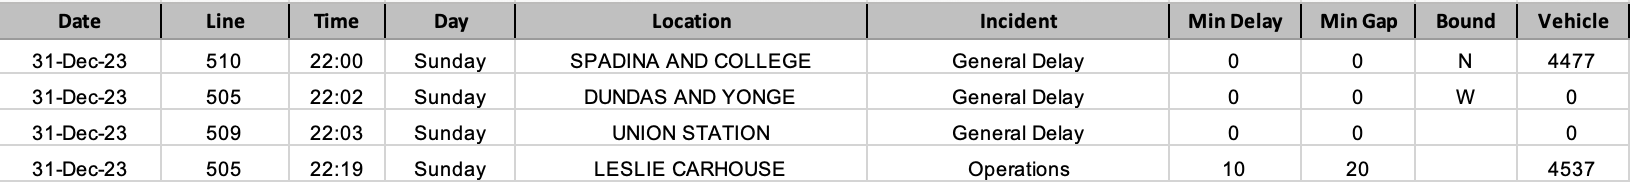
\includegraphics[width=1.0\textwidth]{Figure1.png}
    \captionsetup{skip=0.75em}
    \caption{Zeros and nulls appeared in TTC's 2013 streetcar delay data.}
    \vspace{1em}
    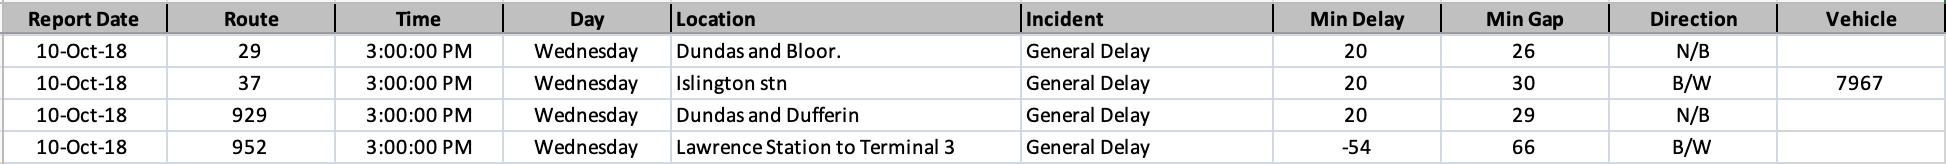
\includegraphics[width=1.0\textwidth]{Figure2.png}
    \captionsetup{skip=0.75em}
    \caption{Negative values appeared in TTC's 2018 bus delay data.}
    \vspace{1em}
    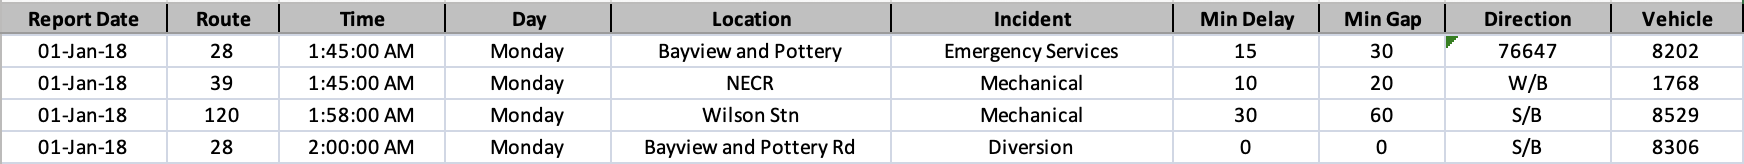
\includegraphics[width=1.0\textwidth]{Figure3.png}
    \captionsetup{skip=0.75em}
    \caption{Incorrect values and the noticeable ratio between Min Delay and Min Gap appeared in TTC's 2018 bus delay data.}
\end{figure}

Therefore, this report will visualize the data quality issues and provide some suggestions
for improving the data quality. As the result, future researchers can access to well-structured 
data and make better decisions.
\end{spacing}

\vspace{-0.25em}
\section{Methodology}
\vspace{-0.25em}
\begin{spacing}{1.2}
This study is quantitative in nature. First of all, we downloaded the raw data from Toronto's 
Open Data and merged them into a single CSV file in each year. We collected all the delayed events
in buses and streetcars from 2014 to April 2026. Then, we used Python to clean the data and visualize 
the data quality issues. Specifically, we used the following libraries:
\begin{itemize}
    \item \texttt{pathlib}: To merge all the raw data into a single CSV file in each year and manage the file paths.
    \vspace{-0.5em}
    \item \texttt{matplotlib, numpy}: To visualize the data quality issues.
\end{itemize}

After that, we analyzed the rate of rows with zero or null values in different columns such as Min 
Delay, Min Gap, Bound, and Vehicle, across the years. In addition, we calculated the rate of rows 
with the value of Min Delay and Min Gap in a generic ratio such as $1:2$ or $1:1$. At the moment, 
through all the years, there are 776,446 delayed events in buses and 163,010 delayed events in 
streetcars in total. We used a combination of pie charts bar graphs, and line graphs to visualize 
the data quality issues. 
\end{spacing}

\vspace{-0.1em}
\begin{center}
\begin{minipage}[t]{0.475\textwidth}
\begin{tcolorbox}[colback=teal!10, colframe=teal!90, title=Pie Charts, fonttitle=\bfseries, height=5cm, valign=center]
\vfill
\begin{spacing}{1.1}
They show the proportion of rows with zero or null values in multiple columns for each year, 
allowing us to identify potential data quality issues in specific years. Each pie chart has
a title that shows the percentage of rows that has at least one zero, negative, or null value.
\end{spacing}
\vfill
\end{tcolorbox}
\end{minipage}
\hfill
\begin{minipage}[t]{0.475\textwidth}
\begin{tcolorbox}[colback=navyblue!10, colframe=navyblue!90, title=Bar Graphs and Line Graphs, fonttitle=\bfseries, height=5cm, valign=top]
\vfill
\begin{spacing}{1.1}
They show the yearly trend of the proportion of rows with zero or null values across the 
2014--2025 period, as well as the ratio of Min Delay and Min Gap, allowing us to identify 
any patterns or anomalies in the data quality over time and across different vehicle types.
\end{spacing}
\vfill
\end{tcolorbox}
\end{minipage}
\end{center}

\vspace{-0.85em}
\section{Data Sources}
\vspace{-0.25em}
\begin{spacing}{1.2}
The data for this analysis was sourced from Toronto's Open Data portal, specifically the
\href{https://open.toronto.ca/dataset/ttc-bus-delay-data}{TTC Bus Delay Data} and 
\href{https://open.toronto.ca/dataset/ttc-streetcar-delay-data}{TTC Streetcar Delay Data}. 
These datasets cover the years 2014 through April 2026, providing a comprehensive view of delay 
events over this period. Each dataset includes multiple columns, which are Date/Reported Date,
Line/Route, Time, Day, Location, Incident, Delay code \textit{(since 2025)} Min Delay, Min Gap, 
Bound/Direction, and Vehicle. The data is collected and updated by the Toronto Transit 
Commission (TTC) and is made available to the public for analysis and research purposes.
\end{spacing}

\section{Results}
\vspace{-0.25em}
\subsection{Proportion and table of Null, Zero, or Negative Values by Column}
\vspace{-0.25em}
\subsubsection{TTC Bus Delay Data (2014--2019)}
\vspace{-0.25em}

\begin{figure}[H]
    \centering
    
    % Row 1: 2014 and 2015
    \begin{minipage}[c]{0.3\textwidth}
        \centering
        \vspace{0.2em}
        \begin{tikzpicture}
            \pie[
            color = {min_delay!80, min_gap, direction, lightgray!80, vehicle},
            text = inside,
            radius = 2.15
            ]
            {5.2/,
             14.2/,
             6.5/,
             0.8/,
             73.5/}
        \end{tikzpicture}
        \\ \vspace{0.5em}
        \textbf{2014 (17.68\%)}
    \end{minipage}
    \hfill
    \begin{minipage}[c]{0.3\textwidth}
        \centering
        \vspace{0.2em}
        \begin{tikzpicture}
            \pie[
            color = {min_delay!80, min_gap, direction, lightgray!80, vehicle},
            text = inside,
            radius = 2.15
            ]
            {5.6/,
             12.0/,
             13.2/,
             1.0/,
             68.2/}
        \end{tikzpicture}
        \\ \vspace{0.5em}
        \textbf{2015 (16.66\%)}
    \end{minipage}
    \hfill
    \begin{minipage}[c]{0.3\textwidth}
        \centering
        \vspace{0.2em}
        \begin{tikzpicture}
            \pie[
            color = {min_delay!80, min_gap, direction, lightgray!80, vehicle},
            text = inside,
            radius = 2.15
            ]
            {4.3/,
             8.8/,
             15.2/,
             0.8/,
             70.8/}
        \end{tikzpicture}
        \\ \vspace{0.5em}
        \textbf{2016 (15.05\%)}
    \end{minipage}
    \vspace{1.5em}

    \begin{minipage}[c]{0.3\textwidth}
        \centering
        \vspace{0.2em}
        \begin{tikzpicture}
            \pie[
            color = {min_delay!80, min_gap, direction, lightgray!80, vehicle},
            text = inside,
            radius = 2.15
            ]
            {4.9/,
             9.3/,
             12.9/,
             0.9/,
             72.0/}
        \end{tikzpicture}
        \\ \vspace{0.5em}
        \textbf{2017 (17.99\%)}
    \end{minipage}
    \hfill
    \begin{minipage}[c]{0.3\textwidth}
        \centering
        \vspace{0.2em}
        \begin{tikzpicture}
            \pie[
            color = {min_delay!80, min_gap, direction, lightgray!80, vehicle},
            text = inside,
            radius = 2.15
            ]
            {4.3/,
             8.2/,
             9.5/,
             0.7/,
             77.3/}
        \end{tikzpicture}
        \\ \vspace{0.5em}
        \textbf{2018 (20.22\%)}
    \end{minipage}
    \hfill
    \begin{minipage}[c]{0.3\textwidth}
        \centering
        \vspace{0.2em}
        \begin{tikzpicture}
            \pie[
            color = {incident, min_delay!80, min_gap, direction, lightgray!80, vehicle},
            text = inside,
            radius = 2.15
            ]
            {5.4/,6.9/,7.8/,6.9/,1.0/,72.0/}
        \end{tikzpicture}
        \\ \vspace{0.5em}
        \textbf{2019 (24.82\%)}
    \end{minipage}

    \vspace{2em}
    
    \textbf{Legend:}
    \quad
    \tikz[baseline=(current bounding box.south)] {
        \draw[fill=location] (0,0) rectangle (0.3,0.3);
    } Location
    \quad
    \tikz[baseline=(current bounding box.south)] {
        \draw[fill=min_delay] (0,0) rectangle (0.3,0.3);
    } Min Delay
    \quad
    \tikz[baseline=(current bounding box.south)] {
        \draw[fill=min_gap] (0,0) rectangle (0.3,0.3);
    } Min Gap
    \quad
    \tikz[baseline=(current bounding box.south)] {
        \draw[fill=direction] (0,0) rectangle (0.3,0.3);
    } Direction
    \quad
    \tikz[baseline=(current bounding box.south)] {
        \draw[fill=vehicle] (0,0) rectangle (0.3,0.3);
    } Vehicle
    \quad
    \tikz[baseline=(current bounding box.south)] {
        \draw[fill=incident] (0,0) rectangle (0.3,0.3);
    } Incident
    
    \caption{Proportion of null, zero, or negative values by column for buses (2014--2019).}
    \vspace{-0.5em}
\end{figure}

\begin{table}[H]
    \centering
        \caption{The number of rows with 0/negative (Z/N) or null values by column for buses (2014--2019).}
        \makebox[\textwidth]{%
        \begin{tabular}{|l|c|c|c|c|c|c|c|c|c|c|c|c|}\toprule
            &\multicolumn{2}{c}{\textbf{2014}}&\multicolumn{2}{c}{\textbf{2015}}&\multicolumn{2}{c}{\textbf{2016}}&\multicolumn{2}{c}{\textbf{2017}}&\multicolumn{2}{c}{\textbf{2018}}&\multicolumn{2}{c|}{\textbf{2019}}
            \\\cmidrule(r){2-3}\cmidrule(r){4-5}\cmidrule(r){6-7}\cmidrule(r){8-9}\cmidrule(r){10-11}\cmidrule(r){12-13} 
            &Z/N&Null&Z/N&Null&Z/N&Null&Z/N&Null&Z/N&Null&Z/N&Null\\\midrule
            Location & 1 & 115 & 0 & 142 & 0 & 110 & 0 & 119 & 0 & 116 & 4 & 172\\
            Min Delay   & 983 & 20 & 811 & 3 & 555 & 2 & 676 & 7 & 579 & 123 & 932 & 254\\
            Min Gap     & 2,701 & 34 & 1,732 & 5 & 1,136 & 8 & 1,299 & 7 & 890 & 452 & 974 & 367\\
            Direction   & 2 & 1,242 & 7 & 1,905 & 1 & 1,960 & 6 & 1,803 & 1 & 1,554 & 1 & 1,183\\
            Vehicle     & 184 & 13,963 & 31 & 9380 & 71 & 9,086 & 51 & 10,030 & 72 & 12,568 & 309 & 12,104\\
            Incident    & 0 & 0 & 0 & 0 & 0 & 0 & 0 & 0 & 0 & 0 & 0 & 935\\\midrule
            Total values & \multicolumn{2}{c|}{19,245} & \multicolumn{2}{c|}{14,016} & \multicolumn{2}{c|}{12,929} & \multicolumn{2}{c|}{13,998} & \multicolumn{2}{c|}{16,355} & \multicolumn{2}{c|}{17,235}\\
            \bottomrule
        \end{tabular}%
        }
\end{table} 


\subsubsection{TTC Bus Delay Data (2020--April 2026)}
\vspace{-0.25em}
\vspace{-0.25em}
\begin{figure}[htbp]
    \centering
    
    % Row 1: 2014 and 2015
    \begin{minipage}[c]{0.3\textwidth}
        \centering
        \vspace{0.2em}
        \begin{tikzpicture}
            \pie[
            color = {line/route, min_delay!80, min_gap, direction, lightgray!80, vehicle},
            text = inside,
            radius = 2.25
            ]
            {0.9/,17.3/,18.3/,28.2/,0.2/,35.1/}
        \end{tikzpicture}
        \\ \vspace{0.5em}
        \textbf{2020 (17.65\%)}
    \end{minipage}
    \hfill
    \begin{minipage}[c]{0.3\textwidth}
        \centering
        \vspace{0.2em}
        \begin{tikzpicture}
            \pie[
            color = {min_delay!80, min_gap, direction, line/route, vehicle},
            text = inside,
            radius = 2.25
            ]
            {14.6/,
             15.4/,
             47.6/,
             1.6/,
             20.9/}
        \end{tikzpicture}
        \\ \vspace{0.5em}
        \textbf{2021 (23.78\%)}
    \end{minipage}
    \hfill
    \begin{minipage}[c]{0.3\textwidth}
        \centering
        \vspace{0.2em}
        \begin{tikzpicture}
            \pie[
            color = {min_delay!80, min_gap, direction, line/route, vehicle},
            text = inside,
            radius = 2.25
            ]
            {12.4/,
             14.0/,
             46.2/,
             1.7/,
             25.6/}
        \end{tikzpicture}
        \\ \vspace{0.5em}
        \textbf{2022 (25.24\%)}
    \end{minipage}
    \vspace{1.5em}

    \begin{minipage}[c]{0.3\textwidth}
        \centering
        \vspace{0.2em}
        \begin{tikzpicture}
            \pie[
            color = {min_delay!80, min_gap, direction, line/route, vehicle},
            text = inside,
            radius = 2.25
            ]
            {21.0/,
             21.9/,
             43.6/,
             2.6/,
             11.0/}
        \end{tikzpicture}
        \\ \vspace{0.5em}
        \textbf{2023 (23.88\%)}
    \end{minipage}
    \hfill
    \begin{minipage}[c]{0.3\textwidth}
        \centering
        \vspace{0.2em}
        \begin{tikzpicture}
            \pie[
            color = {min_delay!80, min_gap, direction, line/route, vehicle},
            text = inside,
            radius = 2.25
            ]
            {25.5/,26.0/,36.1/,2.4/,10.1/}
        \end{tikzpicture}
        \\ \vspace{0.5em}
        \textbf{2024 (24.72\%)}
    \end{minipage}
    \hfill
    \begin{minipage}[c]{0.3\textwidth}
        \centering
        \vspace{0.2em}
        \begin{tikzpicture}
            \pie[
            color = {min_delay!80, min_gap, direction, line/route, vehicle},
            text = inside,
            radius = 2.25
            ]
            {24.8/,25.3/,37.3/,2.4/,10.3/}
        \end{tikzpicture}
        \\ \vspace{0.5em}
        \textbf{Since 2025 (27.17\%)}
    \end{minipage}
    
    \vspace{2em}
    
    \textbf{Legend:}
    \quad
    \tikz[baseline=(current bounding box.south)] {
        \draw[fill=location] (0,0) rectangle (0.3,0.3);
    } Location
    \quad
    \tikz[baseline=(current bounding box.south)] {
        \draw[fill=min_delay] (0,0) rectangle (0.3,0.3);
    } Min Delay
    \quad
    \tikz[baseline=(current bounding box.south)] {
        \draw[fill=min_gap] (0,0) rectangle (0.3,0.3);
    } Min Gap
    \quad
    \tikz[baseline=(current bounding box.south)] {
        \draw[fill=direction] (0,0) rectangle (0.3,0.3);
    } Direction
    \quad
    \tikz[baseline=(current bounding box.south)] {
        \draw[fill=vehicle] (0,0) rectangle (0.3,0.3);
    } Vehicle
    \quad
    \tikz[baseline=(current bounding box.south)] {
        \draw[fill=line/route] (0,0) rectangle (0.3,0.3);
    } Line/Route
    
    \caption{Null, zero, or negative values by column for buses (2020--April 2026).}
\end{figure}

\begin{table}[H]
    \centering
    \captionsetup{width=1.2\textwidth,justification=centering,singlelinecheck=false}
    \caption{The number of rows with 0/negative (Z/N) or null values by column for Buses (2020--April 2026).}
        \makebox[\textwidth]{%
        \begin{tabular}{|l|c|c|c|c|c|c|c|c|c|c|c|c|}\toprule
            &\multicolumn{2}{c}{\textbf{2020}}&\multicolumn{2}{c}{\textbf{2021}}&\multicolumn{2}{c}{\textbf{2022}}&\multicolumn{2}{c}{\textbf{2023}}&\multicolumn{2}{c}{\textbf{2024}}&\multicolumn{2}{c|}{\textbf{Since 2025}}
            \\\cmidrule(r){2-3}\cmidrule(r){4-5}\cmidrule(r){6-7}\cmidrule(r){8-9}\cmidrule(r){10-11}\cmidrule(r){12-13} 
            &Z/N&Null&Z/N&Null&Z/N&Null&Z/N&Null&Z/N&Null&Z/N&Null\\\midrule
            Location & 0 & 47 & 0 & 0 & 0 & 0 & 0 & 0 & 0 & 0 & 0 & 0\\
            Min Delay   & 138 & 4 & 2,242 & 0 & 2,818 & 0 & 4,590 & 0 & 6,733 & 0 & 8,710 & 0\\
            Min Gap     & 251 & 7 & 2,369 & 0 & 3,180 & 0 & 4,801 & 0 & 6,874 & 0 & 8,881 & 0\\
            Direction   & 2 & 2,518 & 1 & 7,304 & 0 & 10,480 & 1 & 9,540 & 1 & 9,531 & 0 & 13,098\\
            Vehicle     & 882 & 2,259 & 3,203 & 0 & 5,802 & 0 & 2,403 & 0 & 2,657 & 0 & 3,622 & 0\\
            Line/Route   & 0 & 78 & 0 & 240 & 0 & 384 & 0 & 570 & 5 & 662 & 0 & 833\\\midrule
            Total values & \multicolumn{2}{c|}{8,941} & \multicolumn{2}{c|}{15,359} & \multicolumn{2}{c|}{22,664} & \multicolumn{2}{c|}{21,905} & \multicolumn{2}{c|}{26,463} & \multicolumn{2}{c|}{35,144}\\
            \bottomrule
        \end{tabular}%
        }
\end{table} 

\subsubsection{TTC Streetcar Delay Data (2014--2019)}
\vspace{-0.25em}
\vspace{-0.25em}
\begin{figure}[htbp]
    \centering
    
    % Row 1: 2014 and 2015
    \begin{minipage}[c]{0.3\textwidth}
        \centering
        \vspace{0.2em}
        \begin{tikzpicture}
            \pie[
            color = {min_delay!80, min_gap, direction, lightgray!80, vehicle},
            text = inside,
            radius = 2.25
            ]
            {11.1/,20.2/,0.9/,1.3/,66.4/}
        \end{tikzpicture}
        \\ \vspace{0.5em}
        \textbf{2014 (9.97\%)}
    \end{minipage}
    \hfill
    \begin{minipage}[c]{0.3\textwidth}
        \centering
        \vspace{0.2em}
        \begin{tikzpicture}
            \pie[
            color = {min_delay!80, min_gap, direction, lightgray!80, vehicle},
            text = inside,
            radius = 2.25
            ]
            {16.4/,
             22.3/,
             1.4/,
             3.0/,
             56.9/}
        \end{tikzpicture}
        \\ \vspace{0.5em}
        \textbf{2015 (11.04\%)}
    \end{minipage}
    \hfill
    \begin{minipage}[c]{0.3\textwidth}
        \centering
        \vspace{0.2em}
        \begin{tikzpicture}
            \pie[
            color = {min_delay!80, min_gap, direction, lightgray!80, vehicle},
            text = inside,
            radius = 2.25
            ]
            {17.0/,
             19.1/,
             1.4/,
             1.8/,
             60.7/}
        \end{tikzpicture}
        \\ \vspace{0.5em}
        \textbf{2016 (9.07\%)}
    \end{minipage}
    \vspace{1.5em}

    \begin{minipage}[c]{0.3\textwidth}
        \centering
        \vspace{0.2em}
        \begin{tikzpicture}
            \pie[
            color = {min_delay!80, min_gap, direction, lightgray!80, vehicle},
            text = inside,
            radius = 2.25
            ]
            {13.3/,
             15.1/,
             1.3/,
             2.1/,
             68.2/}
        \end{tikzpicture}
        \\ \vspace{0.5em}
        \textbf{2017 (10.47\%)}
    \end{minipage}
    \hfill
    \begin{minipage}[c]{0.3\textwidth}
        \centering
        \vspace{0.2em}
        \begin{tikzpicture}
            \pie[
            color = {min_delay!80, min_gap, direction, lightgray!80, vehicle},
            text = inside,
            radius = 2.25
            ]
            {16.4/,17.0/,9.2/,7.6/,49.9/}
        \end{tikzpicture}
        \\ \vspace{0.5em}
        \textbf{2018 (6.24\%)}
    \end{minipage}
    \hfill
    \begin{minipage}[c]{0.3\textwidth}
        \centering
        \vspace{0.2em}
        \begin{tikzpicture}
            \pie[
            color = {min_delay!80, min_gap, direction, lightgray!80, vehicle},
            text = inside,
            radius = 2.25
            ]
            {26.8/,35.4/,12.2/,2.5/,23.1/}
        \end{tikzpicture}
        \\ \vspace{0.5em}
        \textbf{2019 (5.68\%)}
    \end{minipage}
    
    \vspace{2em}
    
    \textbf{Legend:}
    \quad
    \tikz[baseline=(current bounding box.south)] {
        \draw[fill=location] (0,0) rectangle (0.3,0.3);
    } Location
    \quad
    \tikz[baseline=(current bounding box.south)] {
        \draw[fill=min_delay] (0,0) rectangle (0.3,0.3);
    } Min Delay
    \quad
    \tikz[baseline=(current bounding box.south)] {
        \draw[fill=min_gap] (0,0) rectangle (0.3,0.3);
    } Min Gap
    \quad
    \tikz[baseline=(current bounding box.south)] {
        \draw[fill=direction] (0,0) rectangle (0.3,0.3);
    } Direction
    \quad
    \tikz[baseline=(current bounding box.south)] {
        \draw[fill=vehicle] (0,0) rectangle (0.3,0.3);
    } Vehicle
    \caption{Null, zero, or negative values by column for streetcars (2014--2019).}
\end{figure}

\begin{table}[H]
    \centering
        \captionsetup{width=1.2\textwidth,justification=centering,singlelinecheck=false}
        \caption{The number of rows with 0/negative (Z/N) or null values by column for Streetcars (2014--2019).}
        \makebox[\textwidth]{%
        \begin{tabular}{|l|c|c|c|c|c|c|c|c|c|c|c|c|}\toprule
            &\multicolumn{2}{c}{\textbf{2014}}&\multicolumn{2}{c}{\textbf{2015}}&\multicolumn{2}{c}{\textbf{2016}}&\multicolumn{2}{c}{\textbf{2017}}&\multicolumn{2}{c}{\textbf{2018}}&\multicolumn{2}{c|}{\textbf{2019}}
            \\\cmidrule(r){2-3}\cmidrule(r){4-5}\cmidrule(r){6-7}\cmidrule(r){8-9}\cmidrule(r){10-11}\cmidrule(r){12-13} 
            &Z/N&Null&Z/N&Null&Z/N&Null&Z/N&Null&Z/N&Null&Z/N&Null\\\midrule
            Location    & 0 & 17 & 0 & 53 & 0 & 28 & 0 & 36 & 0 & 92 & 0 & 24\\[2pt]
            Min Delay   & 138 & 4 & 287 & 2 & 270 & 2 & 224 & 4 & 161 & 37 & 230 & 28\\[2pt]
            Min Gap     & 251 & 7 & 391 & 1 & 303 & 3 & 257 & 2 & 163 & 43 & 281 & 60\\[2pt]
            Direction   & 1 & 11 & 0 & 24 & 0 & 22 & 0 & 22 & 1 & 0 & 0 & 118\\[2pt]
            Vehicle     & 8 & 840 & 11 & 988 & 72 & 899 & 77 & 1,091 & 10 & 591 & 0 & 223\\\midrule
            Total values & \multicolumn{2}{c|}{1,277} & \multicolumn{2}{c|}{1,757} & \multicolumn{2}{c|}{1,599} & \multicolumn{2}{c|}{1,713} & \multicolumn{2}{c|}{1,098} & \multicolumn{2}{c|}{964}\\
            \bottomrule
        \end{tabular}%
        }
\end{table}

\subsubsection{TTC Streetcar Delay Data (2020--April 2026)}
\vspace{-0.25em}
\vspace{-0.25em}
\begin{figure}[H]
    \centering
    \begin{minipage}[c]{0.3\textwidth}
        \centering
        \vspace{0.2em}
        \begin{tikzpicture}
            \pie[
            color = {line/route, min_delay!80, min_gap, direction, lightgray!80, vehicle},
            text = inside,
            radius = 2.25
            ]
            {2.2/,22.8/,26.0/,31.5/,0.9/,16.6/}
        \end{tikzpicture}
        \\ \vspace{0.5em}
        \textbf{2020 (17.65\%)}
    \end{minipage}
    \hfill
    \begin{minipage}[c]{0.3\textwidth}
        \centering
        \vspace{0.2em}
        \begin{tikzpicture}
            \pie[
            color = {min_delay!80, min_gap, direction, line/route, vehicle},
            text = inside,
            radius = 2.25
            ]
            {13.3/,13.7/,45.9/,1.5/,25.5/}
        \end{tikzpicture}
        \\ \vspace{0.5em}
        \textbf{2021 (23.78\%)}
    \end{minipage}
    \hfill
    \begin{minipage}[c]{0.3\textwidth}
        \centering
        \vspace{0.2em}
        \begin{tikzpicture}
            \pie[
            color = {min_delay!80, min_gap, direction, line/route, vehicle},
            text = inside,
            radius = 2.25
            ]
            {13.0/,
             14.2/,
             43.2/,
             0.6/,
             29.0/}
        \end{tikzpicture}
        \\ \vspace{0.5em}
        \textbf{2022 (25.24\%)}
    \end{minipage}
    \vspace{1.5em}

    \begin{minipage}[c]{0.3\textwidth}
        \centering
        \vspace{0.2em}
        \begin{tikzpicture}
            \pie[
            color = {min_delay!80, min_gap, direction, line/route, vehicle},
            text = inside,
            radius = 2.25
            ]
            {26.8/,
             29.3/,
             31.6/,
             1.8/,
             10.6/}
        \end{tikzpicture}
        \\ \vspace{0.5em}
        \textbf{2023 (23.88\%)}
    \end{minipage}
    \hfill
    \begin{minipage}[c]{0.3\textwidth}
        \centering
        \vspace{0.2em}
        \begin{tikzpicture}
            \pie[
            color = {min_delay!80, min_gap, direction, line/route, vehicle},
            text = inside,
            radius = 2.25
            ]
            {31.0/,31.7/,26.9/,2.0/,8.4/}
        \end{tikzpicture}
        \\ \vspace{0.5em}
        \textbf{2024 (24.72\%)}
    \end{minipage}
    \hfill
    \begin{minipage}[c]{0.3\textwidth}
        \centering
        \vspace{0.2em}
        \begin{tikzpicture}
            \pie[
            color = {min_delay!80, min_gap, direction, line/route, vehicle},
            text = inside,
            radius = 2.25
            ]
            {30.2/,30.7/,27.9/,2.0/,9.2/}
        \end{tikzpicture}
        \\ \vspace{0.5em}
        \textbf{Since 2025 (27.17\%)}
    \end{minipage}
    
    \vspace{2em}
    
    \textbf{Legend:}
    \quad
    \tikz[baseline=(current bounding box.south)] {
        \draw[fill=location] (0,0) rectangle (0.3,0.3);
    } Location
    \quad
    \tikz[baseline=(current bounding box.south)] {
        \draw[fill=min_delay] (0,0) rectangle (0.3,0.3);
    } Min Delay
    \quad
    \tikz[baseline=(current bounding box.south)] {
        \draw[fill=min_gap] (0,0) rectangle (0.3,0.3);
    } Min Gap
    \quad
    \tikz[baseline=(current bounding box.south)] {
        \draw[fill=direction] (0,0) rectangle (0.3,0.3);
    } Direction
    \quad
    \tikz[baseline=(current bounding box.south)] {
        \draw[fill=vehicle] (0,0) rectangle (0.3,0.3);
    } Vehicle
    \quad
    \tikz[baseline=(current bounding box.south)] {
        \draw[fill=line/route] (0,0) rectangle (0.3,0.3);
    } Line/Route
    \caption{Null, zero, or negative values by column for streetcars (2020--April 2026).}
\end{figure}

\begin{table}[H]
    \centering
        \captionsetup{width=1.2\textwidth,justification=centering,singlelinecheck=false}
        \caption{The number of rows with 0/negative (Z/N) or null values by column for Streetcars (2020--April 2026).}
        \makebox[\textwidth]{%
        \begin{tabular}{|l|c|c|c|c|c|c|c|c|c|c|c|c|}\toprule
            &\multicolumn{2}{c}{\textbf{2020}}&\multicolumn{2}{c}{\textbf{2021}}&\multicolumn{2}{c}{\textbf{2022}}&\multicolumn{2}{c}{\textbf{2023}}&\multicolumn{2}{c}{\textbf{2024}}&\multicolumn{2}{c|}{\textbf{Since 2025}}
            \\\cmidrule(r){2-3}\cmidrule(r){4-5}\cmidrule(r){6-7}\cmidrule(r){8-9}\cmidrule(r){10-11}\cmidrule(r){12-13} 
            &Z/N&Null&Z/N&Null&Z/N&Null&Z/N&Null&Z/N&Null&Z/N&Null\\\midrule
            Location    & 0 & 14 & 0 & 0 & 0 & 0 & 0 & 0 & 0 & 0 & 0 & 0\\[2pt]
            Min Delay   & 355 & 2 & 790 & 0 & 915 & 0 & 1,899 & 0 & 2,455 & 0 & 3,489 & 0\\[2pt]
            Min Gap     & 401 & 5 & 810 & 0 & 1,005 & 0 & 2,075 & 0 & 2,509 & 0 & 3,557 & 0\\[2pt]
            Direction   & 0 & 492 & 0 & 2,726 & 0 & 3,049 & 0 & 2,240 & 0 & 2,128 & 0 & 3,231\\[2pt]
            Vehicle     & 210 & 50 & 1,515 & 0 & 2,050 & 0 & 749 & 0 & 666 & 0 & 1,065 & 0\\[2pt]
            Line/Route  & 0 & 35 & 0 & 92 & 0 & 43 & 0 & 128 & 0 & 156 & 0 & 230\\[2pt]\midrule
            Total values & \multicolumn{2}{c|}{1,564} & \multicolumn{2}{c|}{5,933} & \multicolumn{2}{c|}{7,062} & \multicolumn{2}{c|}{7,091} & \multicolumn{2}{c|}{7,914} & \multicolumn{2}{c|}{11,572}\\
            \bottomrule
        \end{tabular}%
        }
\end{table}

\subsubsection{Interpreting and analyzing the results from section 4.1.1 to 4.1.4}
\vspace{0.25em}
\begin{center}
    \begin{minipage}[t]{\textwidth}
    \begin{tcolorbox}[colback=brickred!10, colframe=brickred!90, title=Note: How to correctly interpret the pie charts?, fonttitle=\bfseries, valign=center]
    \vfill
    \begin{spacing}{1.2}
    Each pie chart shows the proportion of cells with zero, negative (Z/N), or null values in multiple columns for a given year.
    Each category is calculated by dividing the number of unknown values in a column by the total number of unknown values 
    in the whole dataset.
    \end{spacing}
    \vfill
    \end{tcolorbox}
    \end{minipage}
\end{center}
\vspace{-0.5em}

\begin{spacing}{1.2}
From 2014 to 2017, both types of vehicles show a similar pattern of proportions of zero, negative (Z/N), 
or null values across the columns. The vehicle column shows the highest proportion of unknown values, 
while the line/route and location columns show the lowest proportion of unknown values. In TTC Bus Delay 
Data, around 70\% of all the unknown values in each year's dataset are in the vehicle column. This
proportion is consistent until 2019. In TTC Streetcar Delay Data, around 60\% to 65\% of all the unknown 
values are in the vehicle column. This proportion significantly decreases to 50\% and 23\% in 2018 and 2019 
respectively. After that, the proportion of unknown values in the vehicle column in both types of vehicles
is gradually decreasing, where it is around 20\% to 30\% in 2020 to 2023 and around 10\% in 2024 to April 2026.
Therefore, it can be concluded that recording the vehicle number is a manual process and may not be important
for the analysis of delay data.
\vspace{0.75em}

In the proportions of Z/N or null values that are in the Min Delay or Min Gap columns, they are roughly the 
same across the years, except from 2014 to 2016 in TTC Bus Delay Data and 2014 and 2019 in TTC Streetcar 
Delay Data. This means that it is more common for both values to be zero, negative or null in one delay event.
In TTC Bus Delay Data, both columns show an increasing trend after 2019, while in TTC Streetcar Delay Data, 
the trend is more fluctuating across the years. This means that the data quality is decreasing since in the
year 2019 and after 2022 in both types of vehicles, the proportion of unknown values in the Min Delay 
and Min Gap columns is significantly higher than before, around 25\% to 30\%.
\vspace{0.75em}

In the proportions of Z/N or null values that are in the Direction column, both types of vehicles show
a similar pattern across the years. Before 2020, the proportion of unknown values is always less than 16\%
in both types of vehicles. Especially in TTC Streetcar Delay Data, the proportion of unknown values 
is always less than 3\%. After 2020, this proportion increases significantly, reaching around 25\% to 30\%
on average and up to 48\% in 2021 to 2023 in Buses and 2021 to 2022 in Streetcars. As a result, the direction
of a vehicle is either poorly recorded or not important since there are several bus routes that only runs 
on one direction.
\vspace{0.75em}

Finally, the proportions of Z/N or null values that are in the Line/Route column or Location column
only appear in the smallest proportion of unknown values in all the columns. This means that there has
been some error in recording the events, since these values are easy to record and check. Additionally, 
these 2 values can be easily recorded automatically by the system.
\end{spacing}

\subsection{Proportion of rows with at least one zero, negative, or null value by year}
\vspace{-0.5em}
\begin{figure}[H]
    \centering
    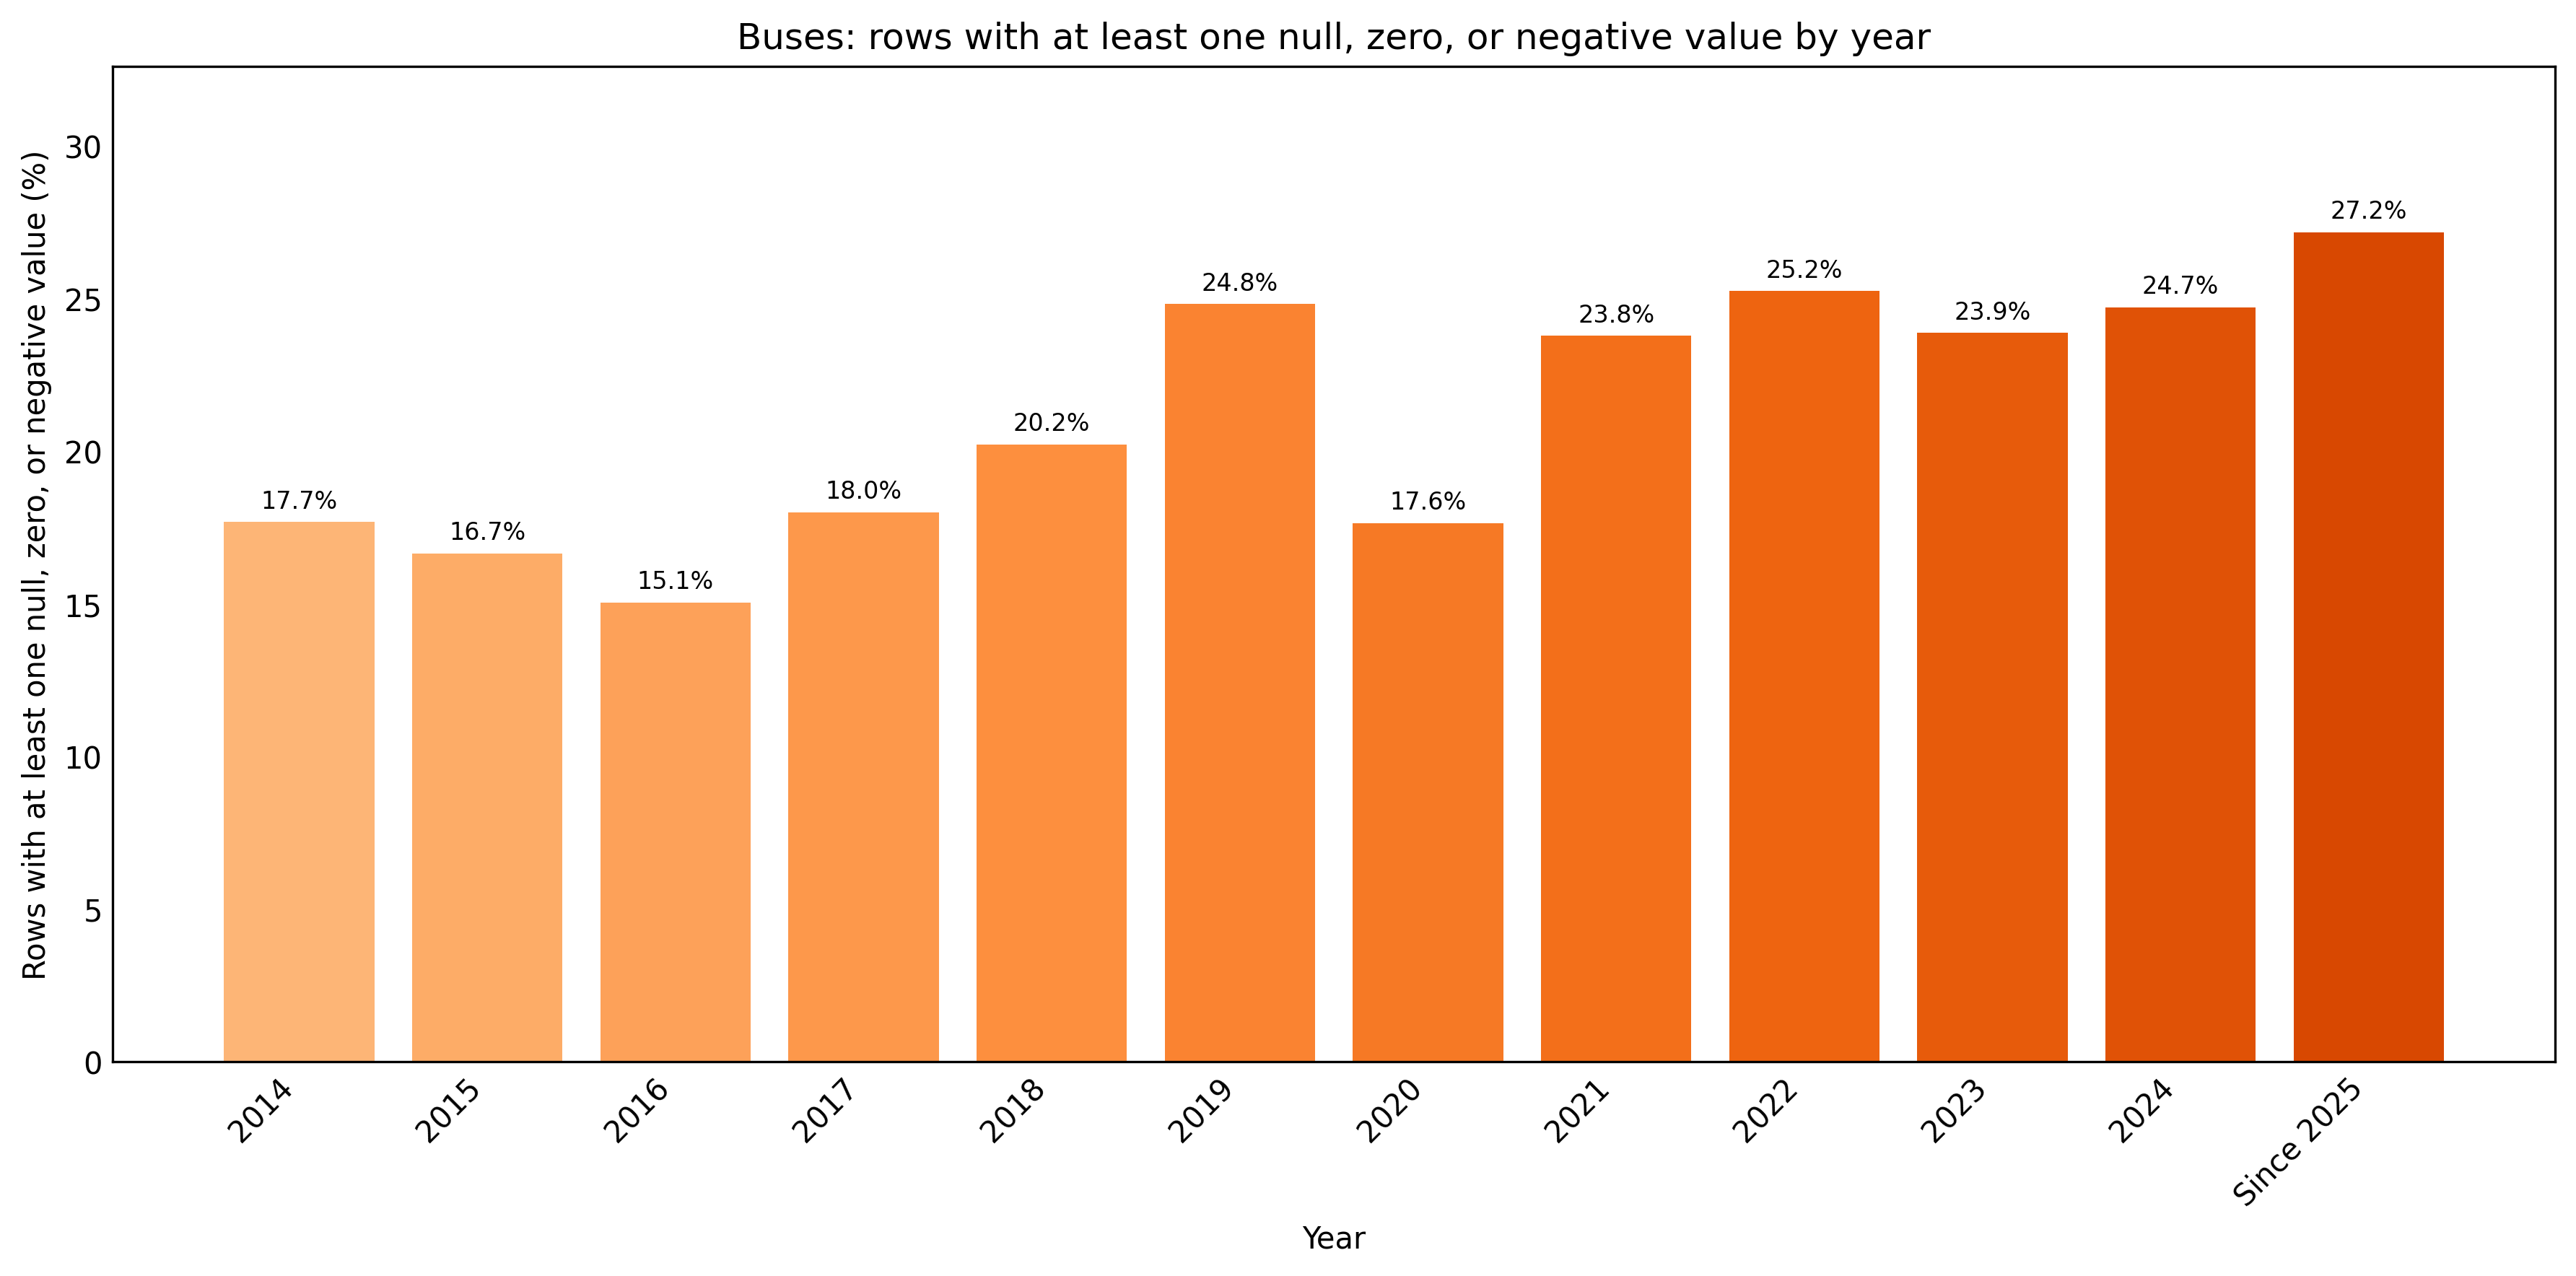
\includegraphics[width=\textwidth]{Buses/null_zero_negative_row_percentage_by_year.png}
    \caption{Yearly percentage of rows with at least one zero, negative, or null value in TTC Buses.}
    \label{fig:yearly-bar-graphs-buses}
\end{figure}
\vspace{-1em}
\begin{figure}[H]
    \centering
    
\includegraphics[width=\textwidth]{Streetcars/null_zero_negative_row_percentage_by_year.png}
    \caption{Yearly percentage of rows with at least one zero, negative, or null value in TTC Streetcars.}
    \label{fig:yearly-bar-graphs-streetcars}
\end{figure}
\vspace{-0.5em}
\begin{spacing}{1.2}
Both bar graphs show a significant increase in the percentage of rows with at least one zero, negative, or null value in the later years.
In TTC Bus Delay Data, the percentage is slowly increasing throughout the years, and the latest year has the highest percentage of 27.2\%.
In TTC Streetcar Delay Data, the percentage of rows with at least one unknown value is relatively low from 2014 to 2020,
mostly between 5\% and 12\%, then rises after that, which is between 25\% and 30\%.
\end{spacing}

\subsection{Proportion of rows with a generic ratio of Min Delay to Min Gap}
\vspace{0.25em}
\begin{center}
    \begin{minipage}[t]{\textwidth}
    \begin{tcolorbox}[colback=darkblue!10, colframe=darkblue, title=Our observations, fonttitle=\bfseries, valign=center]
    \vfill
    \begin{spacing}{1.2}
    Besides noticing a common ratio of Min Delay to Min Gap as $1:2$, we also noticed that the ratio is somtimes 
    $1:1$ or $1:3$. The line graphs below show the percentage of rows with a generic ratio of Min Delay to Min Gap
    out of total rows recorded in each year.
    \end{spacing}
    \vfill
    \end{tcolorbox}
    \end{minipage}
\end{center}
\vspace{-0.75em}
\begin{figure}[H]
    \centering
    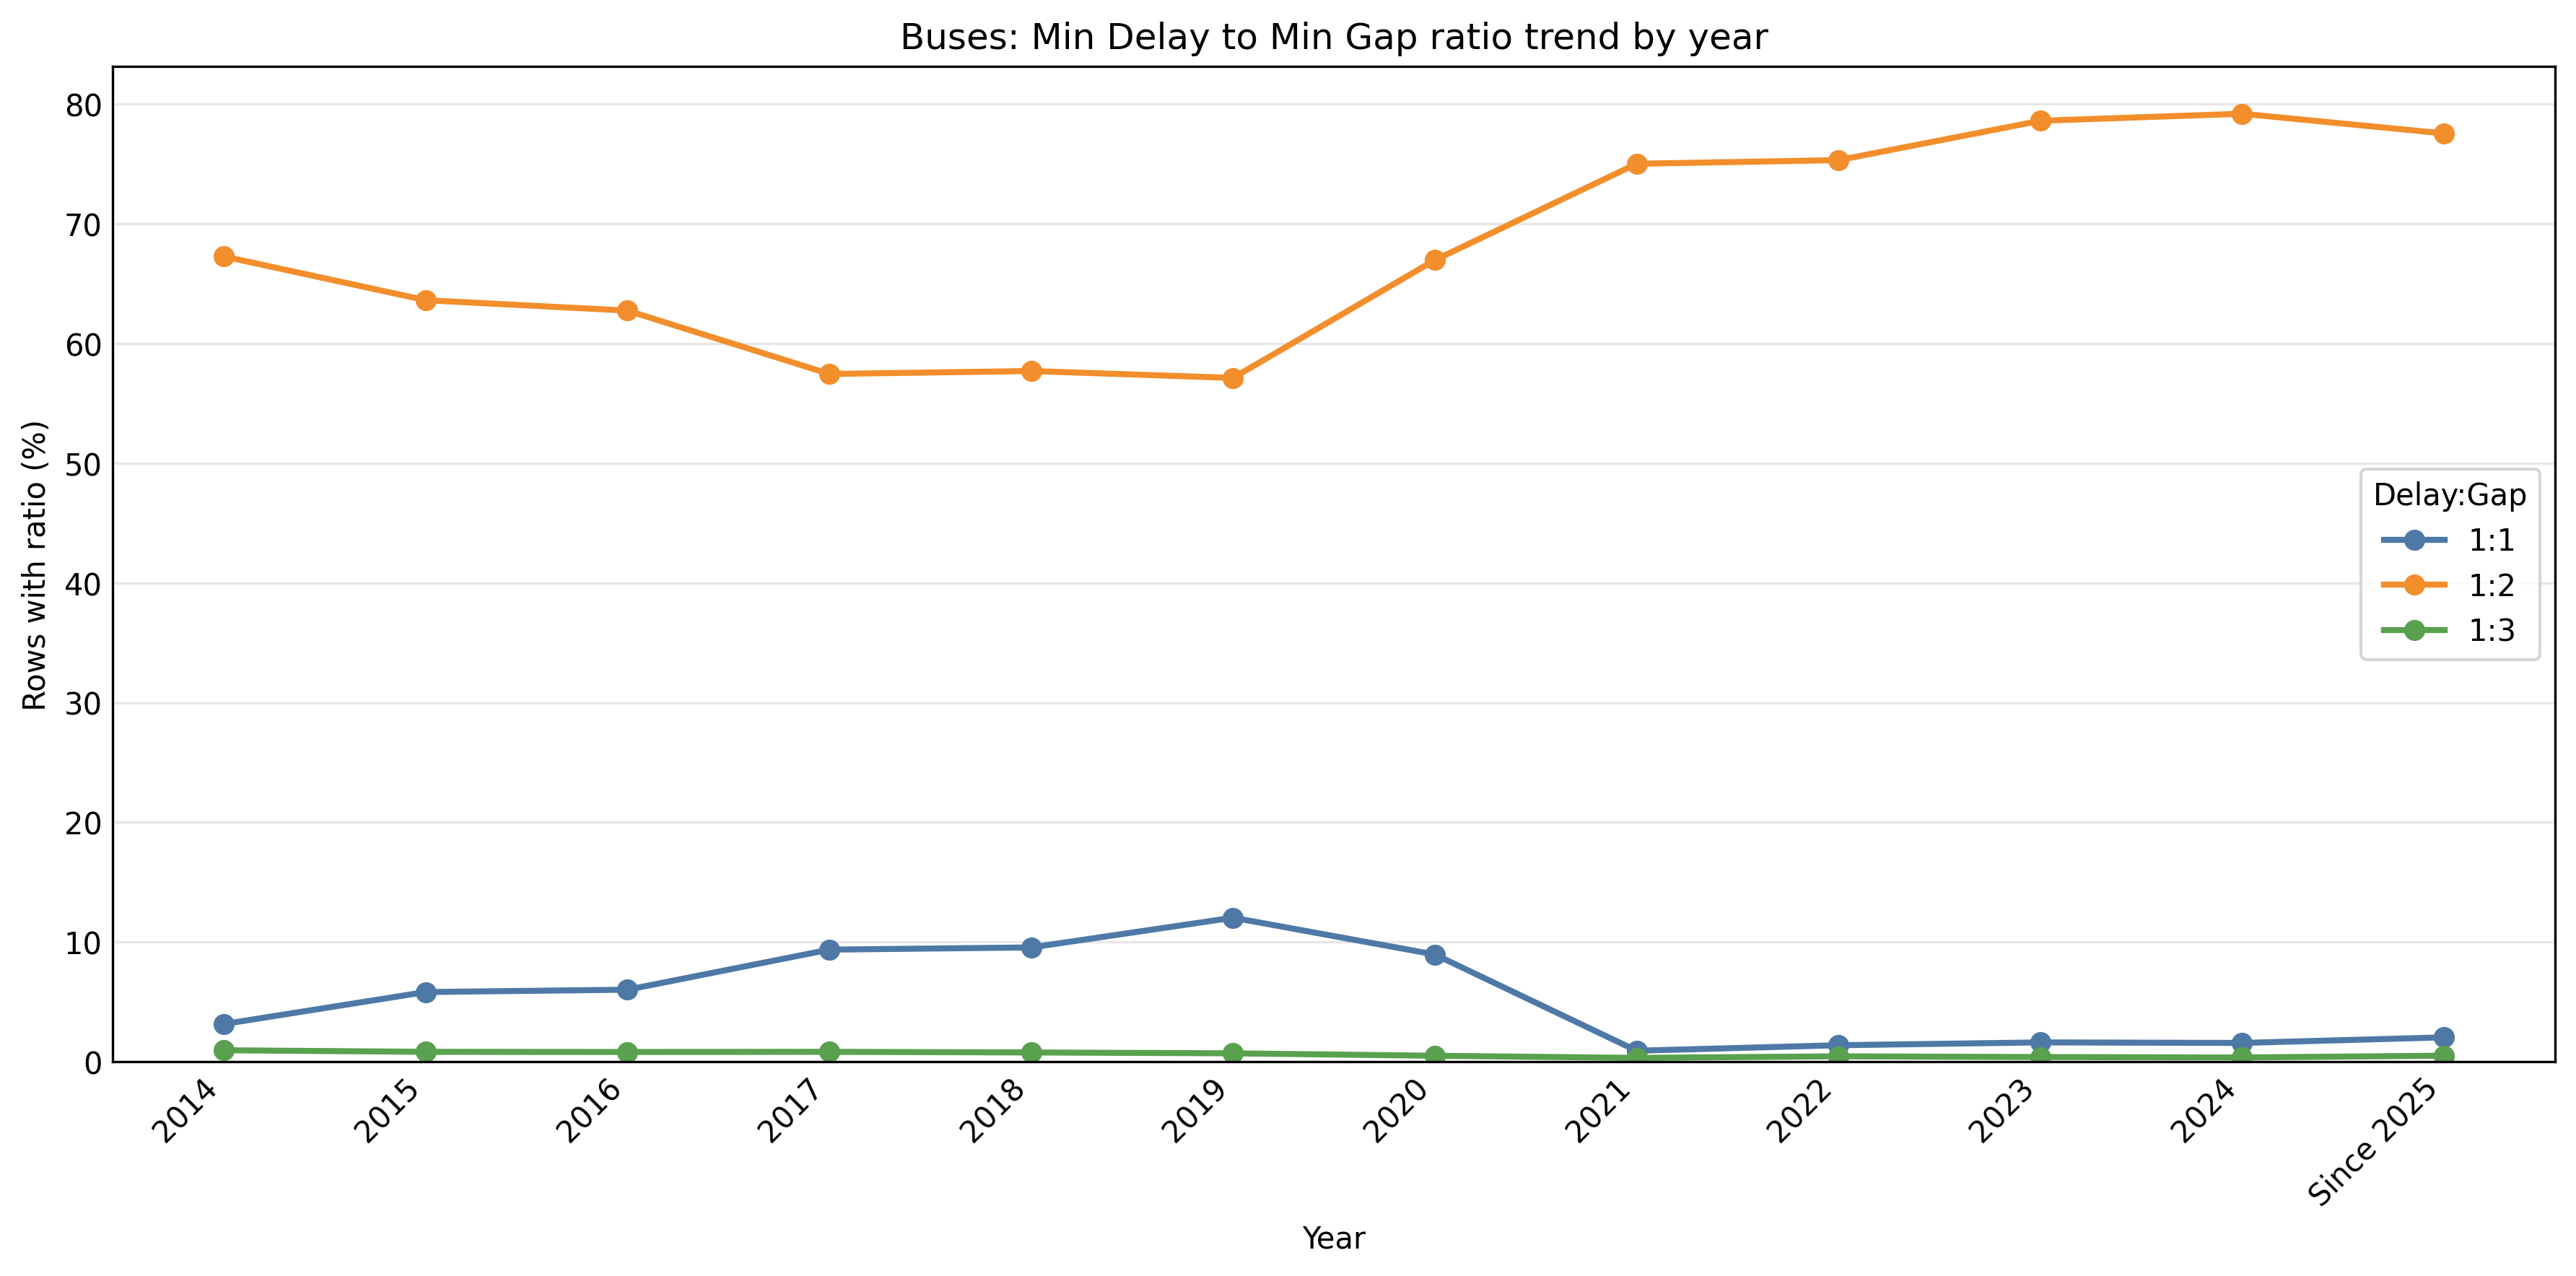
\includegraphics[width=\textwidth]{Buses/delay_gap_ratio_percentage_by_year.png}
    \caption{Yearly percentage of rows with a generic ratio of Min Delay to Min Gap in TTC Buses.}
    \label{fig:yearly-bar-graphs-buses-min-delay-to-min-gap}
\end{figure}
\vspace{-1em}
\begin{figure}[H]
    \centering
    
\includegraphics[width=\textwidth]{Streetcars/delay_gap_ratio_percentage_by_year.png}
    \caption{Yearly percentage of rows with a generic ratio of Min Delay to Min Gap in TTC Streetcars.}
    \label{fig:yearly-bar-graphs-streetcars-min-delay-to-min-gap}
\end{figure}
\vspace{-0.5em}
\begin{spacing}{1.2}
Both line graphs show the majority of ratio $1:2$ in both TTC Buses and Streetcars delay data. In TTC Buses,
the percentage of rows with this ratio $1:2$ varies from 60\% to 80\% throughout the years, while it varies 
from 50\% to 70\% in TTC Streetcars. On the other hand, the percentage of rows with ratio $1:1$ or $1:3$ 
is significantly low, mostly less than 10\% in both types of vehicles. On average, the percentage of rows 
with ratio $1:1$ is around 3\% in TTC Streetcars and around 4\% in TTC Buses and ratio $1:3$ is around 1\% 
in TTC Streetcars and around 2\% in TTC Buses.
\end{spacing}

\vspace{-0.25em}
\section{Limitations}
\vspace{-0.5em}
\begin{spacing}{1.2}
Through our analysis, we have identified several limitations in the TTC delay data. First of all, we only
collected public dataset from \href{https://open.toronto.ca/dataset}{Toronto Open Data Portal}, which is 
a public dataset portal for the City of Toronto. Therefore, the data might not be comprehensive for the public
and there might not be a proper process to collect all the data from the TTC. Second, the data is
not consistent across the years. For example, in TTC Bus Delay Data on July and August 2021, all the
delayed events recorded are for the Streetcars, and they are identical to the Streetcars delay data on 
July and August 2021. This means that the data is not always accurate and there might be some errors in the 
data. Finally, there are 2 verions of column names for recording the minutes of delay and gap, which are 
Min Delay \& Min Gap and Delay \& Gap. The second version appeared in 2020, which raises a question about
whether the minutes recorded in Delay \& Gap have the same meaning as the minutes recorded in Min Delay \& Min Gap.
\end{spacing}

\vspace{-0.25em}
\section{Conclusion}
\vspace{-0.5em}
\begin{spacing}{1.2}
\subsection{Overall Data Quality Assessment}
\vspace{-0.25em}
The data quality is poor and worsening. Across the full 2014--April 2026 period covering
776,446 bus and 163,010 streetcar delay events, the proportion of records containing at least one
zero, negative, or null value has grown from approximately 15--18\% in the mid-2010s to 27.2\%
for buses and 34.5\% for streetcars in the most recent data. No corrective trend is visible in
either series after 2019. The root cause is structural: the current system relies on operators
entering free-form text with little or no automated validation, and the data schema has been
revised multiple times without backward-compatible versioning or a published changelog. The 
dataset is not ready for predictive modelling and requires substantial cleaning before
even descriptive analysis is reliable.
\end{spacing}
\vspace{-0.25em}

\subsection{Proposed Data Collection and Management Process}
\vspace{-0.5em}

\begin{spacing}{1.2}
The core principle is that any field a machine can record automatically should never require human text entry.
Therefore, we propose the following data collection and management process:
\end{spacing}
\vspace{-0.5em}
\subsubsection{Track 1: Automatic Data Capture from On-Board Sensors}
\vspace{-0.25em}
\begin{spacing}{1.2}
    TTC buses and streetcars already carry Computer-Aided Dispatch and Automatic Vehicle Location
    (CAD/AVL) systems, GPS receivers, and door-open sensors. These systems should automatically
    populate the following fields without any operator input.
    
    \begin{itemize}[leftmargin=2em]
        \item \textbf{Date and Time:} Sourced from the system clock at the moment the delay event is
        created.
        \item \textbf{Route and Vehicle ID:} Pulled from the CAD/AVL assignment at the time of the event.
        \item \textbf{Location:} Resolved from the GPS coordinates to the nearest GTFS stop ID, providing a
        stable, unambiguous reference rather than a free-text location name.
        \item \textbf{Direction:} Derived from the trip pattern registered in the CAD/AVL system, constrained
        to the four valid values: N/B, S/B, E/B, W/B.
        \item \textbf{Min Delay:} Calculated automatically as the difference between the scheduled departure
        time and the actual departure time, both of which CAD/AVL records.
        \item \textbf{Min Gap:} Derived from the real headway to the following vehicle, also available from
        AVL. This field must never be a manual entry or a formula of the delay value; it should
        reflect an independent measurement.
    \end{itemize}
\end{spacing}
\vspace{-0.5em}
\subsubsection{Track 2: Constrained Operator Input}
\vspace{-0.25em}
\begin{spacing}{1.2}
Only fields that genuinely require operator judgment should be entered manually. The operator
interface should be a mobile application presenting the following two inputs only. In addition,
an optional free-text notes field may be included for supplementary context, but its contents
must not be stored in any column used for quantitative analysis.
    
\begin{itemize}[leftmargin=2em]
    \item \textbf{Incident type:} A dropdown menu populated with the current approved vocabulary.
    Free-text entry must not be permitted. The vocabulary should be versioned (see
    Section~6.2.5).
    \item \textbf{Start/End Delay:} The operator taps ``start delay'' when an event begins and ``end
    delay'' when it clears. This provides a manual timing cross-check against the AVL-derived
    figure and requires no text entry.
\end{itemize}
\end{spacing}
\vspace{-0.5em}

\subsubsection{Validation Layer}
\vspace{-0.25em}
\begin{spacing}{1.2}
Before any record is written to the database, an automated validation step must enforce the
following rules. Records failing any of these checks must be routed to a reject queue for 
supervisor review. They must not be silently written to the database with invalid values.
Therefore, the validation layer is a crucial step to ensure the data accuracy.
\end{spacing}
\vspace{-0.5em}
\begin{spacing}{1.2}
\begin{itemize}[leftmargin=2em, itemsep=3pt, topsep=3pt, parsep=0pt]
    \item $\texttt{Min Delay} \geq 0$ and $\texttt{Min Gap} \geq 0$.
    \item \texttt{Direction} is one of N/B, S/B, E/B, or W/B.
    \item \texttt{Route} and \texttt{Vehicle} are non-null integers matching the current fleet and route registry.
    \item \texttt{Incident} is a value from the currently approved vocabulary.
    \item The record is not a duplicate of an existing event within five minutes on the same route.
\end{itemize}
\end{spacing}
\vspace{-0.5em}

\subsubsection{Central Database and Unique Event Identifier}
\vspace{-0.25em}
\begin{spacing}{1.2}
Every confirmed event must be assigned a system-generated unique identifier (\texttt{EventID}) at
write time. This is the single most important structural change: it makes deduplication
unambiguous, enables external systems to reference specific events, and allows corrections to be
linked to their originals without overwriting history. The database should be an append-only log;
corrections are new records linked to the original by \texttt{EventID}, not in-place overwrites.
\end{spacing}
\vspace{-0.25em}
\subsubsection{Schema Versioning and Open Data Release}
\vspace{-0.25em}
\begin{spacing}{1.2}
Column names, data types, and the incident vocabulary must be treated as a versioned schema.
Any change to these elements increments the schema version number and is published in a
human-readable changelog alongside the corresponding data release. Consumers of the data can
then detect schema changes programmatically and update their pipelines accordingly.
\vspace{0.75em}

As an immediate remediation, the column names should be standardised to \texttt{Min Delay} and
\texttt{Min Gap} as the canonical form across all years, with the 2020-onward data backfilled to use
these names.
\end{spacing}
\vspace{-0.25em}
\subsubsection{Nightly Data Quality Audit}
\vspace{-0.25em}
\begin{spacing}{1.2}
An automated job should run each night over the previous day's records and flag the following
conditions for supervisor review.
\end{spacing}
\vspace{-0.5em}
\begin{spacing}{1.2}
\begin{itemize}[leftmargin=2em, itemsep=3pt, topsep=4pt, parsep=0pt]
    \item Records where $\texttt{Min Gap} = 2 \times \texttt{Min Delay}$ (suggesting formula fill rather than
    independent measurement).
    \item Records where $\texttt{Min Delay} = 0$.
    \item Routes with a null rate in \texttt{Direction} exceeding a configurable threshold (e.g., 10\%).
    \item Any \texttt{Incident} value not present in the current approved vocabulary (catching
    typographical variants and ad-hoc additions before they propagate).
\end{itemize}
\end{spacing}
\vspace{-0.25em}
\begin{spacing}{1.2}
Flagged records are surfaced in a supervisor dashboard rather than removed. The raw history is
preserved; the flags are stored separately and linked by \texttt{EventID}.
\end{spacing}
\end{document}